\scanpage{13}
\diagram{\begin{tikzcd}[ampersand replacement=\&,column sep=small]
\mathbb H^*(X,M^\bullet)\simeq\mathbb H^*(X,Q^*[M^\bullet])\&
E_2^{pq}=\mathbb H^p(X,C^\bullet(V^q))\arrow[l,Rightarrow]
\end{tikzcd}}
(\unsure{réf} à EGA $\underline O_{\mathrm{III}}$ ?). On peut encore l'écrire, en posant par définition, pour un Module stratifié $\underline{\unsure{V}}$ relativement à $S$,
\[
H^p(X_{\inserted{\mathrm{str}}}\deleted{\unsure{/S}},\underline V)
=\mathbb H^p(X,C^\bullet_{\mathrm{str}}(\underline V)),
\]
sous la forme
\diagram{\[\boxed{\begin{gathered}
\begin{tikzcd}[ampersand replacement=\&,column sep=small]
\mathbb H^*(X,M^\bullet)\&E_2^{pq}=H^p_{\deleted{\unsure{\mathrm{str}}}}(X_{\inserted{\mathrm{str}}},V^q(M^\bullet))\arrow[l,Rightarrow]
\end{tikzcd}\\[1em]
\text{où}\qquad V^q(M^\bullet)=\mathcal H^q(Q^0[M^\bullet])
\end{gathered}}\]}

\uline{Corollaire} Supposons que l'on ait
\[
V^q(M^\bullet)=0\quad\text{pour}\quad q\neq q_0
\]
alors on a des isom canoniques
\[
\mathbb H^n(X,M^\bullet)\simeq H^{n-q_0}_{\mathrm{str}}(X,V^{q_0}(M^\bullet))
\]
\margin{\figure{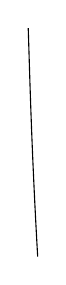
\begin{tikzpicture}[x=1cm,y=1cm]
\draw (0,0) .. controls (-.08,1.4) and (-.1,2.3) .. (-.12,2.9);
\end{tikzpicture}}}
Ceci montre, \inserted{supposant p.ex. que $q_0=0$,} que le premier \unsure{mb}
\margin{12}
